\chapter{Einleitung}
\label{chap:einleitung}
Heutzutage ist die Menschheit darauf fokussiert, die komplette Welt zu digitalisieren. Dabei
existiert ein Grundsatz, alles, was digitalisiert werden kann, soll digitalisiert werden. Um dies
zu realisieren, ist es von Nöten, überall Hardware und Software zu verbinden. Sei es nun das
Handy, mit welchem durch nur einem klick die Bankdaten angezeigt werden können, oder ein
selbstfahrendes Auto, welches einen Anwender selbstständig zum Ziel fährt. Dies sind nur zwei
Bespiele von einer unendlich langen Liste. Hinter diesen technischen Wundern stecken meist
mehrere Tausend kleiner Mikrocomputern und Mikrocontrollern, die dann mittels Software zusammen
interagieren. Die Kombination dieser zwei Komponenten werden durch den Oberbegriff „Embedded
System“ oder auch zu Deutsch ein „Eingebettetes System“ definiert.
\newline
\newline
Embedded Systems können dabei grundsätzlich zwischen zwei Plattformen unterschieden werden:
\begin{itemize}
    \item Deeply Embedded System
    \item Open Embedded System
\end{itemize}
\newline
\newline
Deeply Embedded Systems sind die wesentlichen Bausteine des Internet of Things
\cite{HochschuleniederrheimDeeply}. Die Anwendung,
die bei Deeply Embedded Systems implementiert wird, basiert auf speziell angepassten
Echtzeitbetriebssystemen, den Programmiersprachen C oder C++ und ganz speziellen
\ac{gui}-Frameworks wie zum Beispiel TouchGFX.
\newline
\newline
Anders als bei den Deeply Embedded Systems, die sehr auf speziellen Technologien aufbauen, bieten
Open Embedded Systems eine höhere Flexibilität in sachen Technologien an. Dem Programmierer ist
also die Möglichkeit gegeben, unterschiedliche Technologien, als auch unterschiedliche
Programmiersprachen zu verwenden. Dort gilt bis dato die Kombination von C++ und Qt für
\ac{gui}-lastige Systeme als „State of the Art“.
\newline
\newline
Die Konstellation zwischen C++ und Qt hat bislang auch funktioniert, jedoch kommt dieser Ansatz
auch mit Problemen mit sich, denn die höheren Entwicklungszeiten für die Entwicklung von C++
Anwendungen, sowie die geringe Verfügbarkeit von Experten auf dem Arbeitsmarkt sorgen für
schlechtere Qualität und längere Produktionszeiten.
\newline
\newline
Um diesen Problemen zu entgegnen, soll in dieser Abschlussarbeit ein anderer Ansatz betrachtet
werden. Und zwar könnten sowohl die Anwendungsschicht als auch die Persistenzschicht als .Net
Core Anwendungen implementiert werden. Als \ac{gui}-Technologie soll dabei die neue
Microsoft-Technologie namens \emph{Blazor} als Qt Ersatz zum Einsatz kommen. Somit kann erreicht
werden, die komplette Codebasis mit .Net Core auszutauschen und eine Programmier-freundlichere
Umgebung für Entwickler im Open Embedded Systems zu erschaffen.
\section{Aufgabenstellung}
\label{sec:aufgabenstellung}
Das Ziel dieser Arbeit ist die Entwicklung eines Blazor-basierten Frontend auf einem Raspberry Pi
4 um einen aussagekräftigen Vergleich zwischen den Technologien schaffen zu können und um eine
mögliche verdrängung mittels Blazor zu demonstrieren. Dazu soll
zunächst begutachtet werden, wie der momentane Stand der Technik für Open Embedded Systems ist,
um anschließend das gleiche Verhalten mittels Blazor zu reproduzieren. Insbesondere sollen dabei
verschiedene Aspekte, wie zum Beispiel das Verhalten zur Laufzeit, dieses Ansatzes überprüft werden.
\begin{figure}[h]
    \centering
    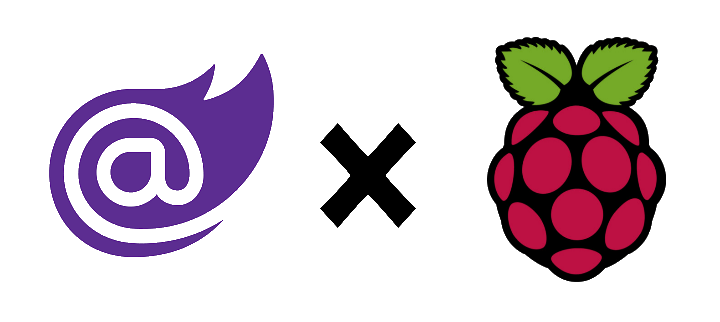
\includegraphics[width=0.8\textwidth, center]{Einleitung/blazorxraspberry}
    \caption[Blazor mit Raspberry Pi]{Blazor mit Raspberry Pi}
    \label{img:blazorxraspberry}
\end{figure}
\section{Verwendete Hardware}
\label{sec:verwendeteHardware}
Als Zielplattform für diese Arbeit dient ein Raspberry Pi 4B. Der Raspberry Pi 4B
verfügt dabei unter anderem über die folgenden technischen Spezifikationen: \cite{RasberryPiSpecs}
\begin{itemize}
    \item 1,5 GHz ARM Cortex-A72 Quad-Core-CPU
    \item 1 GB, 2 GB oder 4 GB LPDDR4 SDRAM
    \item Gigabit LAN RJ45 (bis zu 1000 Mbit)
    \item Bluetooth 5.0
    \item 2x USB 2.0 / 2x USB 3.0
    \item 2x microHDMI (1x 4k @60fps oder 2x 4k @30fps)
    \item 5V/3A @ USB Typ-C
    \item 40 GPIO Pins
    \item Mikro SD-Karten Slot
\end{itemize}
Der Raspberry Pi 4B wird mit dem \emph{Raspbian Buster with desktop} auf der SD-Karte betrieben.
\newline
Um noch mehr Funktionalität aufbringen zu können, wurde auf dem Raspberry Pi ein
\emph{RPI SENSE HAT Shield} aufgesteckt. Mit hilfe des \emph{RPI SENSE HAT Shield} können dann
unter anderem Daten wie zum Beispiel die momentane Temperatur oder auch die momentane
Luftfeuchtigkeit gewonnen werden. Zudem ist auf dem Raspberry Pi noch eine 8x8 LED-Matrix enthalten
und ein Joystick mit 5 Knöpfen, die eingelesen werden können.
\begin{figure}[h]
    \centering
    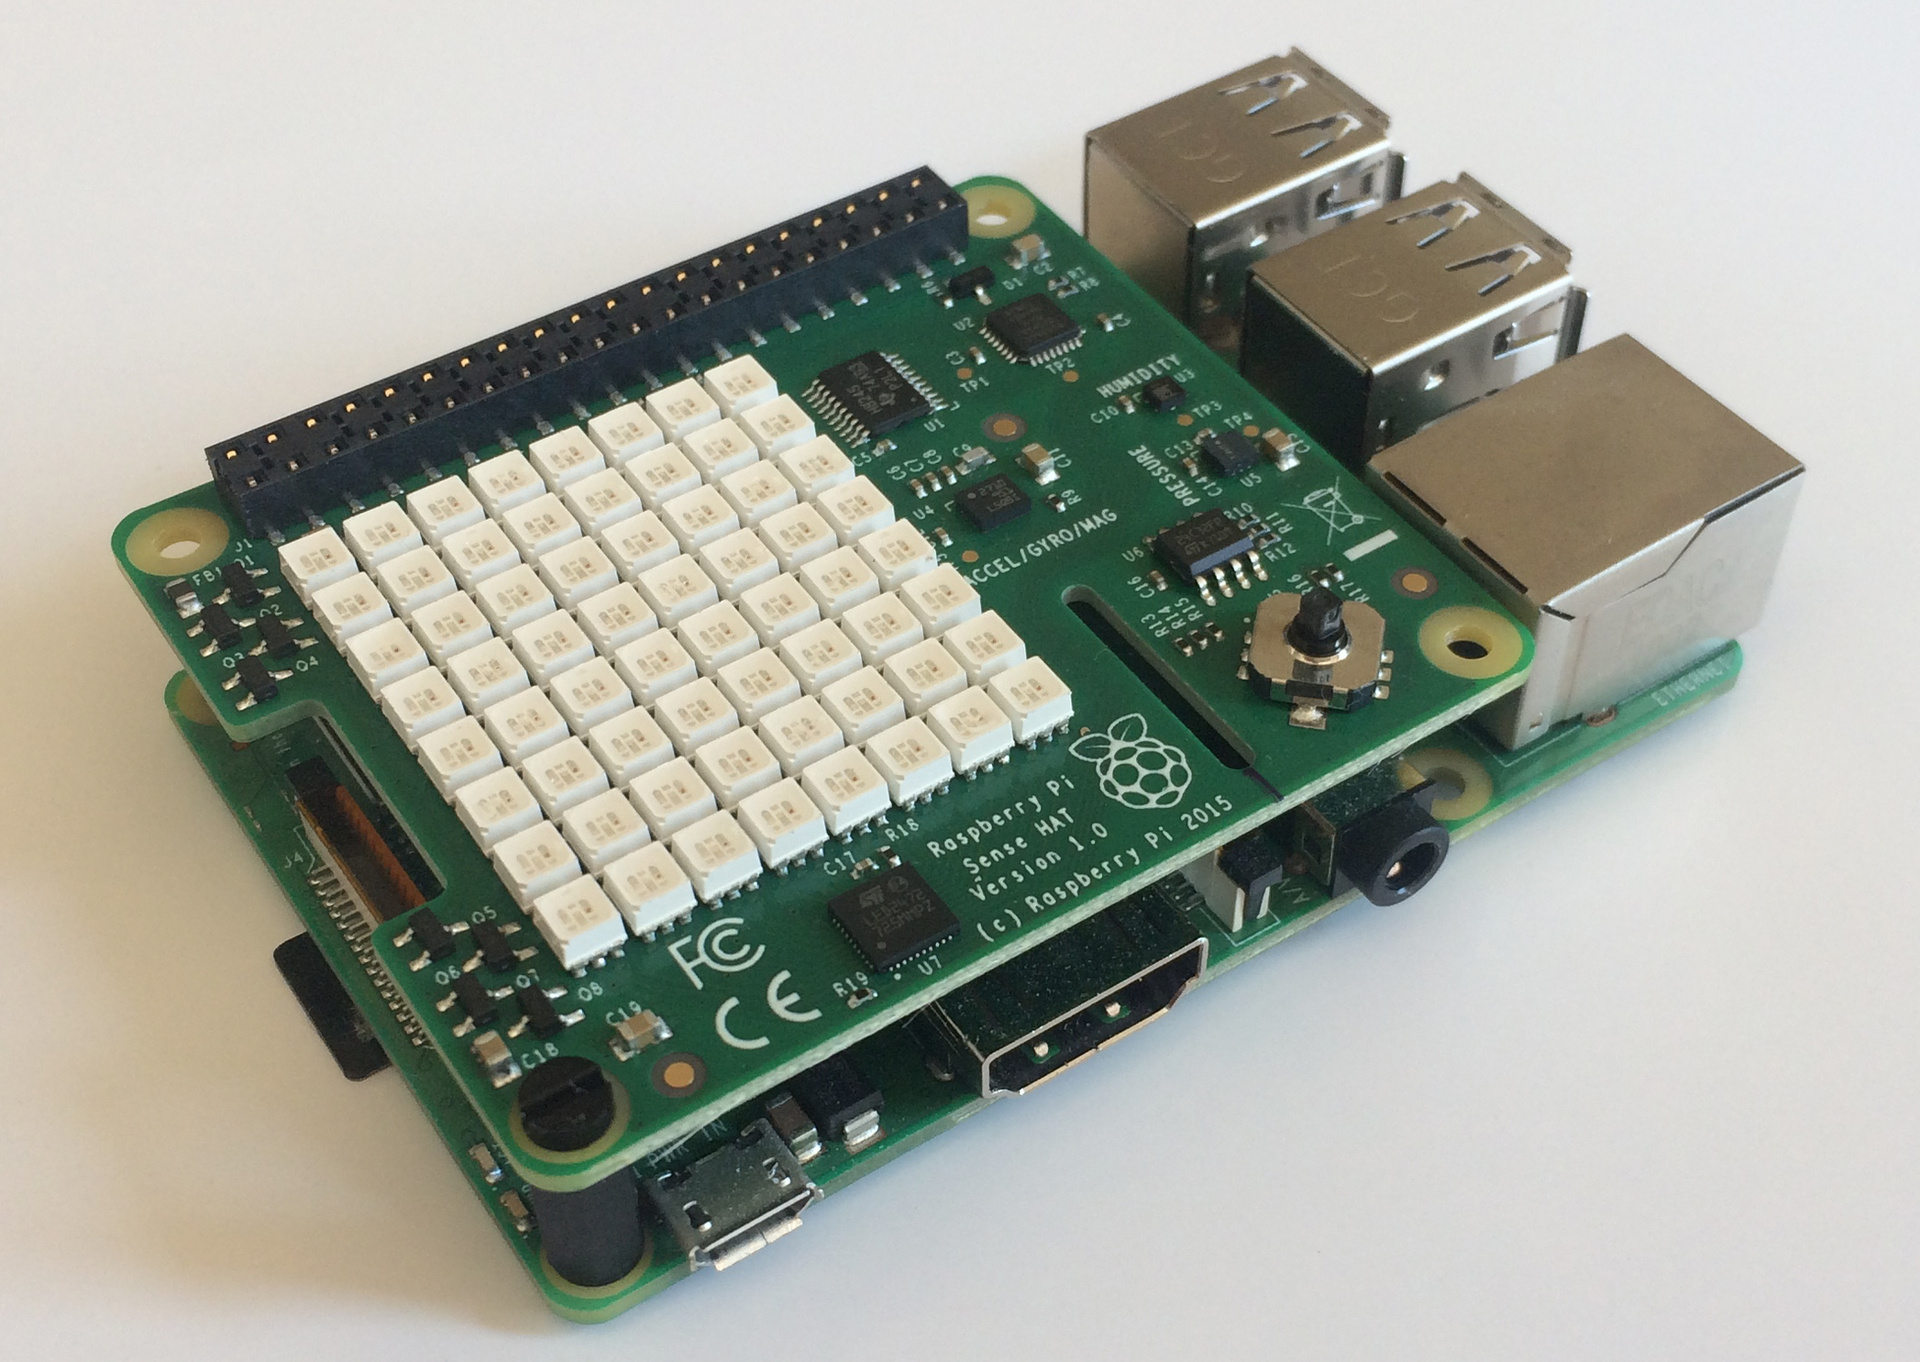
\includegraphics[width=0.5\textwidth, center]{Einleitung/pi-sense}
    \caption[Raspberry Pi 4 B]{Verwendeter Raspberry Pi}
    \label{img:piSense}
\end{figure}


\section{Verwendete Software}
\label{sec:verwendeteSoftware}
Im Rahmen dieser Thesis werden die folgenden Softwaretools zur Entwicklung eingesetzt:
\begin{itemize}
    \item Um eine Visualisierung des Images \emph{Raspbian Buster with desktop} von dem Raspberry
    Pi zu erhalten, wird die Windows Desktop Anwendung \emph{VNC Viewer} verwendet. Dadurch ist
    die Möglichkeit gegeben, bequem und einfach den Raspberry Pi remote zu bedienen.
    \item Für die Demonstrierung des Kapitels \emph{\nameref{chap:standTechnik}} wird eine
    beispielhafte grafische Oberfläche mithilfe des Qt-Creators implementiert.
    \item Den Zugriff auf die Funktionalitäten des \emph{RPI SENSE HAT Shield} wird mittels der
    \emph{RTIMUlib} Bibliothek realisiert.
    \item Die Programmiersprachen dieser Arbeit werden sich hauptsächlich aus \emph{C++} und
    \emph{C\#} beziehungsweise .Net Core zusammensetzen.
    \item Um den Zugriff auf die Funktionalitäten des \emph{RPI SENSE HAT Shield} mittels .Net
    Core zu gewährleisten, wird die Iot Bibliothek von Microsoft verwendet.
    \item Die Implementierung der Anwendung mit Blazor wird dann letztendlich mittels der
    kostenlosen IDE \emph{Visual Studio Code} realisiert.
    \item Um zwischen dem Host Rechner und dem Raspberry Pi Dokumente und Ordner auszutauschen,
    wird die Desktop-Applikation \emph{WinSCP} verwendet.
\end{itemize}

Die oben vorgestellten Tools und Programmiersprachen wurden nicht explizit vorgegeben, sind
dementsprechend auch selbst ausgesucht und sind zu Beginn dieser Thesis auch schon alle komplett
eingerichtet.
